\section{Del 1}

Vi har fundet et lydklip af vindmølle støj med en sampling frekvens på 48kHz og et lydklip af en PC blæser med en sampling frekvens på 44.1kHz. Udvalgte 10 sekunder af disse filer er plottet i \autoref{fig:wm_10s} og \autoref{fig:pc_10s}.

Det kan ses at vindmøllen svinger i lydstyrke ca.\ en gang hvert 1.5 sekund, mens blæseren kører med en mere konstant (og lavere) lydstyrke.

Ud fra sampling frekvenserne kan man beregne frekvensopløsningen med 
\begin{equation}
\Delta f = \frac{f_{sample}}{N}
\end{equation}

For vindmøllen, med $f_{sample}=48000$ bliver det $\Delta f_{wm} = \frac{48000}{480000} = 0.1$Hz.
PC blæseren har samme frekvensopløsning.


\begin{figure}[h]
\centering
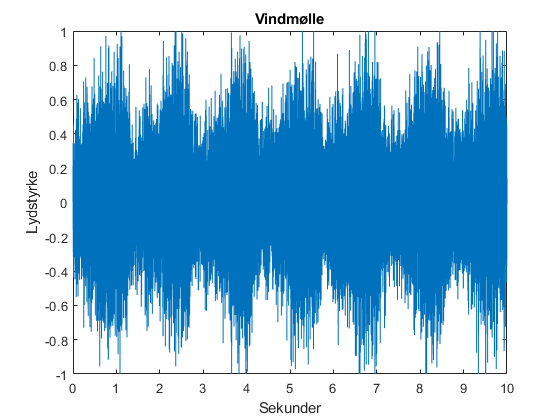
\includegraphics[width=\textwidth]{figures/Windmill_10s}
\caption{10s lyd fra vindmølle}%
\label{fig:wm_10s}
\end{figure}

\newpage

\begin{figure}[h]
\centering
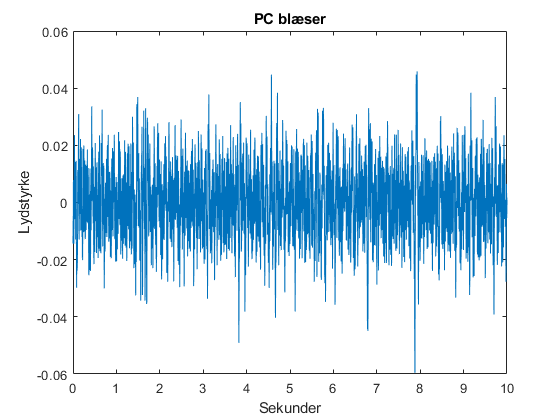
\includegraphics[width=\textwidth]{figures/pcFan_10s}
\caption{10s lyd fra PC blæser}%
\label{fig:pc_10s}
\end{figure}

\newpage
